%%%%%%%%%%%%%%%%%%%%%%%%%%%%%%%%%%%%%%%%%%%%%%%%%%%%%%%%%%%%%%%%%%%%%%%%%%%%%%%%%%%%%%
%%%  Roomba: Automatic Validation, Correction and Generation of Dataset Metadata  %%%%
%%%%%%%%%%%%%%%%%%%%%%%%%%%%%%%%%%%%%%%%%%%%%%%%%%%%%%%%%%%%%%%%%%%%%%%%%%%%%%%%%%%%%%

\documentclass{../../Tools/LaTEX/sig-alternate}

\usepackage{graphics}
\usepackage{listings}
\usepackage{xcolor}
\usepackage{color}
\usepackage{url}
\graphicspath{ {figures/} }

\newtheorem{deflda}{Axiom}
\newcommand{\todo}[1]{\noindent\textcolor{red}{{\bf \{TODO}: #1{\bf \}}}}

\colorlet{punct}{red!60!black}
\definecolor{background}{HTML}{FFFFFF}
\definecolor{delim}{RGB}{20,105,176}

% Language Definitions for JSON
\lstdefinelanguage{json}{
	basicstyle=\tiny,
    numbersep=4pt,
    showstringspaces=false,
    breaklines=true,
    frame=lines,
    literate=
      {:}{{{\color{punct}{:}}}}{1}
      {,}{{{\color{punct}{,}}}}{1}
      {[}{{{\color{delim}{[}}}}{1}
      {]}{{{\color{delim}{]}}}}{1},
}

\permission{Copyright is held by the International World Wide Web Conference Committee (IW3C2). IW3C2 reserves the right to provide a hyperlink to the author's site if the Material is used in electronic media.}
\conferenceinfo{WWW 2015 Companion,}{May 18--22, 2015, Florence, Italy.}
\copyrightetc{ACM \the\acmcopyr}
\crdata{978-1-4503-3473-0/15/05. \\
http://dx.doi.org/10.1145/2740908.2742827}

\clubpenalty=10000
\widowpenalty = 10000

%%%%%%%%%%%%%%%%%%%%%%%%%%%%%%%
%%%  Beginning of document  %%%
%%%%%%%%%%%%%%%%%%%%%%%%%%%%%%%

\begin{document}

\title{Roomba: Automatic Validation, Correction and \\Generation of Dataset Metadata}
\subtitle{Enhancing Dataset Search and Spam Detection}

\numberofauthors{1}
\author{\alignauthor $\dagger\ddagger$ Ahmad Assaf, $\ddagger$ Aline Senart, and $\dagger$ Rapha\"{e}l Troncy \\
\affaddr$\dagger${EURECOM, Sophia Antipolis, France} \\ \affaddr$\ddagger${ SAP Labs, Sophia Antipolis, France} \\
\email{$\dagger$raphael.troncy@eurecom.fr, $\ddagger$firstName.lastName@sap.com}
}

\maketitle

%%%%%%%%%%%%%%%%%%
%%%  Abstract  %%%
%%%%%%%%%%%%%%%%%%

\begin{abstract}
Data is being published by both the public and private sectors and covers a diverse set of domains ranging from life sciences to media or government data. An example is the Linked Open Data (LOD) cloud which is potentially a gold mine for organizations and individuals who are trying to leverage external data sources in order to produce more informed business decisions. Considering the significant variation in size, the languages used and the freshness of the data, one realizes that spotting spam datasets or simply finding useful datasets without prior knowledge is increasingly complicated. In this paper, we propose Roomba, a scalable automatic approach for extracting, validating, correcting and generating descriptive linked dataset profiles. While Roomba is generic, we target CKAN-based data portals and we validate our approach against a set of open data portals including the Linked Open Data (LOD) cloud as viewed on the DataHub. The results demonstrate that the general state of various datasets and groups, including the LOD cloud group, needs more attention as most of the datasets suffer from bad quality metadata and lack some informative metrics that are required to facilitate dataset search.
\end{abstract}

% A category with the (minimum) three required fields
\category{H.3}{Information Storage and Retrieval}{Content Analysis and Indexing}

\keywords{Dataset Profile, Metadata, Data Quality, Linked Data}

%%%%%%%%%%%%%%%%%%%%%%%%%
%%%  1. Introduction  %%%
%%%%%%%%%%%%%%%%%%%%%%%%%

\section{Introduction}
\label{sec:introduction}
\textit{Data profiling} is the process of creating descriptive information and collect statistics about that data. It is a cardinal activity when facing an unfamiliar dataset~\cite{Li:WISM:12}. It helps in assessing the importance of a dataset, in improving users' ability to search and reuse part of a dataset and in detecting irregularities to improve its quality. Data profiling includes typically several tasks:
\begin{itemize}
 \item \textbf{metadata profiling} that provides general information on the dataset (dataset description, release and update dates), legal information (license information, openness), practical information (access points, data dumps);
 \item \textbf{statistical profiling} that provides statistical information about data types and patterns in the dataset, i.e. properties distribution, number of entities and RDF triples;
 \item \textbf{topical profiling} that provides descriptive knowledge on the dataset content and structure, e.g. tags and categories used to facilitate search and reuse.
\end{itemize}

The main entry point for discovering and identifying data\-sets is either through public data portals such as DataHub\footnote{\url{http://datahub.io}}, the Europe's Public Data\footnote{\url{http://publicdata.eu}} or private data search engines such as Quandl\footnote{\url{https://quandl.com/}}, Engima\footnote{\url{http://enigma.io/}}. Data on public portals is checked manually as administrators review, validate and correct data\-sets information and attach suitable metadata when available. The increasing number of datasets hinders the scalability of this process, affecting the correct and efficient spotting of datasets spam. CKAN-based data portals rely on metadata attached to datasets that enable search as they run a Solr index on the metadata schemas. Having missing or inconsistent information will affect the search results quality.

In this paper, we propose Roomba, a scalable automatic approach for extracting, validating, correcting and generating descriptive linked dataset profiles. Our framework consists of a processing pipeline that combines techniques for data portals identification, datasets crawling and a set of pluggable modules for the profiling tasks. Roomba validates dataset metadata against an aggregated standard set of information. Metadata fields are automatically corrected when possible, e.g. for adding a missing license URL. Moreover, a report describing all the issues and highlighting those that cannot be automatically fixed is created and sent by email to the dataset's maintainer. There exist various statistical and topical profiling tools for both relational and Linked Data. The architecture of Roomba allows to easily add them as additional profiling modules. However, in this paper, we focus on the task of dataset metadata profiling and present our findings by running Roomba on the LOD cloud\footnote{\url{http://datahub.io/dataset?tags=lod}}. The results demonstrate that the general state of the LOD cloud needs more attention as most of the datasets suffer from bad quality metadata. The noisiest metadata are about the access information such as the license, the resource descriptions as well as problem related to resource availability.

\begin{figure*}[!htbp]
  \centering
  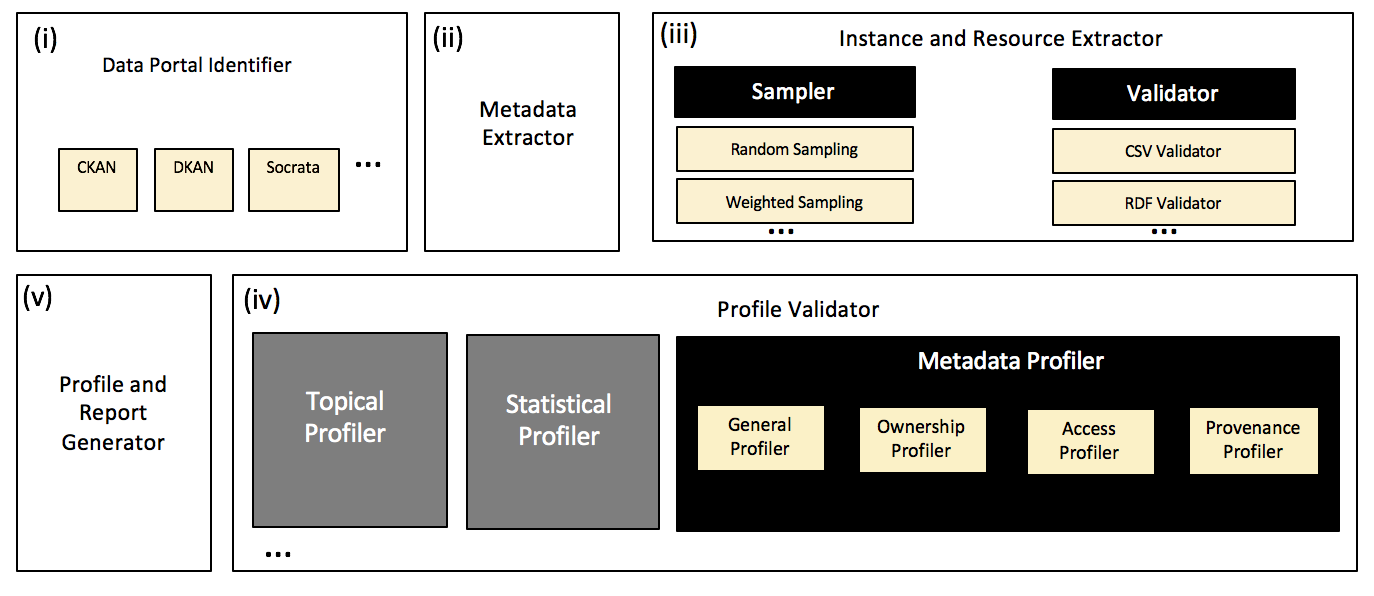
\includegraphics[scale=0.39]{figure-1_architecture.png}
  \caption{Processing pipeline for validating and generating dataset profiles}
  \label{fig:Roomba_architecture}
\end{figure*}

%%%%%%%%%%%%%%%%%%%%%%%%%
%%%  2. Related Work  %%%
%%%%%%%%%%%%%%%%%%%%%%%%%

\section{Related Work}
\label{sec:related-work}
Semantic sitemaps~\cite{Cyganiak:ESWC:08} and RDFStats~\cite{Lanegger:DEXA:09} were one of the first to deal with RDF data statistics and summaries. However, there has been lately a plethora of tools like ExpLOD~\cite{Khatchadourian:ESWC:10}, LODStats~\cite{Auer:EKAW:12}, ProLOD++~\cite{Abedjan:ICDE:14}, LODOP~\cite{Forchhammer:PROFILES:14} and Aether~\cite{Makela:ESWC:14} that compute some statistical information which is vital to applications dealing with query optimization and answering, data cleansing, schema induction and data mining~\cite{Jentzsch:ISWC:14,Lalithsena:WI:13}.

Topical and categorical information facilitates dataset search and reuse. Topical profiling focuses on content-wise analysis at the instances and ontological levels. In~\cite{Lalithsena:WI:13,Bohm:CIKM:12,Fetahu:ESWC:14}, the authors try to automatically infer information about the underlying dataset depending on external knowledge bases or the dataset's internal structure and ontological information.

The Open Data Dashboard project\footnote{\url{http://labs.data.gov/dashboard/}} tracks and measures how US government web sites implement the Open Data principles to understand the progress and current status of their public data listings. A validator analyzes machine readable files (e.g. JSON files) for automated metrics like the number of resolved URLs, HTTP status and content-type. However, deep schema information about the metadata is missing like description, license information or tags. Similarly, on the LOD cloud, the Data Hub LOD Validator\footnote{\url{http://validator.lod-cloud.net/}} gives an overview of Linked Data sources cataloged. It offers a step-by-step validator guidance to check a dataset completeness level for inclusion in the LOD cloud. The results are divided into four different compliance levels from basic to reviewed and included in the LOD cloud. Although it is an excellent tool to monitor LOD compliance, it still lacks the ability to give detailed insights about the completeness of the metadata and an overview on the state of the entire LOD cloud group while being very specific to the LOD cloud group rules and regulations.

%%%%%%%%%%%%%%%%%%%%%%%%%%%%%%%%%%%
%%%  3. Framework Architecture  %%%
%%%%%%%%%%%%%%%%%%%%%%%%%%%%%%%%%%%

\section{Framework Architecture}
\label{sec:framework}
In this section, we provide an overview of the processing steps for validating and generating dataset profiles. Figure~\ref{fig:Roomba_architecture} shows the main steps: (i) data portal identification; (ii) metadata extraction; (iii) instance and resource extraction; (iv) profile validation and (v) profile and report generation.

\subsection{System Overview}
Roomba is built as a Command Line Interface (CLI) application using Node.js. Instructions on installing and running Roomba are available on its public Github repository\footnote{\url{https://github.com/ahmadassaf/opendata-checker}} and explained in this short screencast\footnote{\url{http://youtu.be/p7Y-mDN_Y2s}}. Related functions are encapsulated into modules that can be easily plugged in/out the processing pipeline.

\subsection{Data Portal Identification}
Data portals can be considered as data access points providing tools to facilitate data publishing, sharing, searching and visualization. CKAN is the world's leading open-source data portal platform powering web sites like the DataHub, Europe's Public Data and the U.S Government's open data. Modeled on CKAN, DKAN is a standalone Drupal distribution that is used in various public data portals as well. Identifying the software powering data portals is a vital first step to understand the API calls structure. Web scraping is a technique for extracting data from Web pages. We rely on several scraping techniques in the identification process which includes a combination of the following:
\begin{itemize}
  \item \textbf{URL inspection}: Check the existence of certain URL patterns. Various CKAN-based portals are hosted on sub-domains of \url{http://ckan.net}, for example, CKAN Brazil is at \url{http://br.ckan.net}.
  \item \textbf{Meta tags inspection}: The \texttt{<meta>} tag provides metadata about the HTML document. They are used to specify page description, keywords, author, etc. Inspecting the \texttt{content} attribute can indicate the type of the data portal. We use CSS selectors to check the existence of these meta tags. An example of a query selector is \texttt{meta[content*=`ckan']} (all meta tags with the attribute content containing the string $CKAN$). This selector can identify CKAN portals whereas the \texttt{meta[content*=`Drupal']} can identify DKAN portals.
  \item \textbf{Document Object Model (DOM) inspection}: Similar to the meta tags inspection, we check the existence of certain DOM elements or properties. For example, CKAN-based portals will have DOM elements with class names like \texttt{ckan-icon} or \texttt{ckan-footer-logo}. A CSS selector like \texttt{.ckan-icon} will be able to check if a DOM element with the class name \texttt{ckan-icon} exists. The list of elements and properties to inspect is stored in a separate configurable object for each portal. This allows the addition and removal of elements as deemed necessary.
\end{itemize}

The identification process for each portal can be easily customized by overriding the default function. Moreover, adding or removing steps from the identification process can be easily configured. After those preliminary checks, we query one of the portal's API endpoints. For example, DataHub is identified as CKAN, so we will query the API endpoint at \url{http://datahub.io/api/action/package_list}. A successful request will list the names of the site's datasets, whereas a failing request will signal a possible failure of the identification process.

\subsection{Metadata Extraction}
Data portals expose a set of information about each dataset as metadata. The model used varies across portals. However, a standard model should contain information about the dataset's title, description, maintainer email, update and creation date, etc. We divided the metadata information into the following:

\textbf{General information}: General information about the dataset, e.g. title, description and ID. This general information is manually filled by the dataset owner. In addition to that, tags and group information are required for classification and enhancing dataset discoverability. This information can be entered manually or inferred using modules plugged into the topical profiler.

\textbf{Access information}: Information about accessing and using the dataset. This includes the dataset URL, license information (i.e. license title and URL) and information about the dataset's resources. Each resource has also a set of attached metadata, e.g. resource name, URL, format, size.

\textbf{Ownership information}: Information about the ownership of the dataset, e.g. organization details, maintainer details, author. The existence of this information is important to identify the authority on which the generated report and the newly corrected profile will be sent to.

\textbf{Provenance information}: Temporal and historical information on the dataset and its resources, e.g. creation and update dates, version information. Most of this information can be automatically filled up and tracked.

Although Roomba is generic and accepts any data model to check against, for this demo, we have used the CKAN standard model\footnote{\url{http://demo.ckan.org/api/3/action/package_show?id=adur_district_spending}} as we do our experiments on the LOD cloud. After identifying the underlying portal software, we perform iterative queries to the API in order to fetch datasets metadata and persist them in a file-based cache system. Depending on the portal software, we can issue specific extraction jobs. For example, in CKAN-based portals, we are able to crawl and extract the metadata of a specific dataset, or all the datasets in a specific group (e.g. the LOD Cloud), or all the datasets in the portal.

\subsection{Instance and Resource Extraction}
From the extracted metadata, we are able to identify all the resources associated with that dataset. They can have various types like a SPARQL endpoint, API, file, visualization, etc. However, before extracting the resource instance(s), we perform the following steps:
\begin{itemize}
  \item \textbf{Resource metadata validation and enrichment}: Check the resource attached metadata values. The validation process issue an HTTP request to the resource and automatically fills up various missing information when possible, like the mime type and size by extracting them from the HTTP response header.
  \item \textbf{Format validation}: Validate specific resource formats against a linter or a validator.
\end{itemize}

Considering that some dataset contains large amounts of resources and the limited computation power of some machines on which Roomba might run on, a sampler module is introduced to execute various sample-based strategies discussed in~\cite{Fetahu:ESWC:14} that were found to generate accurate results even with comparably small a sample size of 10\%.

\subsection{Profile Validation}
The metadata validation process identifies missing information and is able to automatically correct them. Each set of metadata (general, access, ownership and provenance) is validated and corrected automatically when possible. Each profiler task has a set of metadata fields to check against. The validation process checks if each field is defined and if the value assigned is valid.

There are special validation steps for various fields. For example, for ownership information where the maintainer email has to be defined, the validator checks if the email field is an actual valid email address. A similar process is done to URLs whenever found and we issue an HTTP \texttt{HEAD} request in order to check whether a URL is reachable or not. For the dataset resources, we use the \texttt{content-header} information when the request is successful in order to extract, compare and correct further metadata values like the mime type and the content size.

From our experiments, we found out that datasets' license information is generally noisy. The license names, if found, are not standardized. For example, Creative Commons CC Zero can be CC0 or CCZero. Moreover, the license URI, if found and if de-referenceable, can point to different reference knowledge bases such as \texttt{\url{http://opendefinition.org}}. To overcome this issue, we have manually created a mapping file standardizing the set of possible license names and the reference knowledge base\footnote{\url{https://github.com/ahmadassaf/opendata-checker/blob/master/util/licenseMappings.json}}. In addition, we have also used the open source and knowledge license information\footnote{\url{https://github.com/okfn/licenses}} to normalize the license information and add additional metadata like the domain, maintainer and open data conformance.

\subsection{Profile and Report Generation}
The validation process highlights the missing information and presents them in a human readable report. The report can be automatically sent to the dataset maintainer email if provided in the metadata. In addition to the generated report, the enhanced profiles are represented in JSON using the CKAN data model and are publicly available\footnote{\url{https://github.com/ahmadassaf/opendata-checker/tree/master/results}}. Data portal administrators need an overall knowledge of the portal datasets and their properties. Roomba has the ability to generate numerous reports of all the datasets by passing formatted queries. There are two main set of aggregation tasks that can be run:
\begin{itemize}
  \item \textbf{Aggregating meta-field values}: Passing a string that corresponds to a valid field in the metadata. The field can be flat like \texttt{license\_title} (aggregates all the license titles used in the portal or in a specific group) or nested like \texttt{resource>resource\_type} (aggregates all the resources types for all the datasets). Such reports are important to have an overview of the possible values used for each metadata field.
  \item \textbf{Aggregating key:object meta-field values}: Passing two meta-field values separated by a colon \texttt{:} (e.g. \texttt{resources>resource\_type:resources>name}). These reports are important as one can aggregate the information needed when also having the set of values associated to it printed.
\end{itemize}

%%%%%%%%%%%%%%%%%%%%%%%%%%%%%%%%%%%%%%%%%
%%%  4. Demonstration and Conclusion  %%%
%%%%%%%%%%%%%%%%%%%%%%%%%%%%%%%%%%%%%%%%%

\section{Demonstration and Conclusion}
During the demo, we will show how one can crawl a data portal, generate reports based on manual queries over the datasets metadata, validate a dataset profile and generate a new enriched profile with automatically fixed some problems. Moreover, users will be invited to try Roomba providing their own datasets hosted on any CKAN-powered portal and directly check the generated report.

Roomba is flexible and extensible. It can be plugged into data portals or used as a standalone tool to check for bad quality dataset metadata and identify possible spam. Automatically corrected profiles are of higher quality thus improving dataset search and retrieval. Further work includes introducing workflows that will be able to correct the rest of the metadata either automatically or through intuitive manually-driven interfaces. We also plan to integrate statistical and topical profilers to be able to generate full comprehensive profiles.

%%%%%%%%%%%%%%%%%%%%%%%%%
%%%  Acknowledgments  %%%
%%%%%%%%%%%%%%%%%%%%%%%%%

\section*{Acknowledgments}
This research has been partially funded by the European Union's 7th Framework Programme via the project Apps4EU (GA No. 325090).
\vspace{0.5cm}

%%%%%%%%%%%%%%%%%%%%%%
%%%  Bibliography  %%%
%%%%%%%%%%%%%%%%%%%%%%

\bibliographystyle{abbrv}
\bibliography{../../Bibliography/bibliography}

% ACM needs 'a single self-contained file'!

%APPENDICES are optional
\balancecolumns
% That's all folks!

\end{document}
